%%%%%%%%%%%%%%%%%%%%%%%%%%%%%%%%%%%%%%%%%%%%%%%%%%%%%%%%%%%%%%%%%%%%%%%%%%%%%%%%
%Objetivo: Propor um conjunto de recomendações de melhorias para as
% 		   as funcionalidade das FGRMs
%Autores: Vagner Clementino <vagnercs@dcc.ufmg.br>
%		  Rodolfo Resende <rodolfo@dcc.ufmg.br>
%Criação: dom fev 26 12:49:27 BRT 2017
%Modificação:: sáb mai 13 14:17:28 -03 2017
%Revisão: dom abr 23 23:16:51 -03 2017
%%%%%%%%%%%%%%%%%%%%%%%%%%%%%%%%%%%%%%%%%%%%%%%%%%%%%%%%%%%%%%%%%%%%%%%%%%%%%%%%
\chapter{Sugestões de Melhorias para FGRMs}
\label{ch:sug_melhoria}

\section{Introdução}
\label{sec:sug_melhoria_intro}

No levantamento descrito no Capítulo~\ref{ch:pesquisa-profissionais} os
profissionais consultados se mostraram, em geral, satisfeitos com as
funcionalidades disponibilizadas pelas FGRMs. Cerca de 90\% dos
par\-ti\-ci\-pan\-tes fizeram uma avaliação positiva da ferramenta que utiliza,
além disso, uma quantidade equivalente disse que recomendariam a FGRM para um
novo projeto.

Não obstante, naquela mesma pesquisa, apresentamos uma lista de possíveis novas
funcionalidades para as FGRMs e perguntamos ao participante se ele sente falta
de alguma. O resultado desta pergunta foi que cerca de 85\% responderam
positivamente, ou seja, os participantes se mostraram interessados na inclusão
de pelo menos uma das funcionalidades propostas nas FGRMs que utilizam. A partir
da análise deste resultado é possível inferir que os desenvolvedores estão
satisfeitos com a ferramenta utilizada, contudo, \textit{não conhecem ou não têm
    acesso ao potencial de funções que este tipo software poderia oferecer}.

Diante do exposto, entendemos que podemos contribuir com o estado a\-tu\-al das
funcionalidades das FGRMs propondo um conjunto de melhorias. As sugestões foram
compiladas utilizando a literatura da área e os resultados obtidos nesta
dissertação, especialmente com base nos
Capítulos~\ref{ch:mapeamento-sistematico} e~\ref{ch:pesquisa-profissionais}, na
Seção~\ref{sec:caracterizacao_ferramentas} e nos estudos que propõem melhorias
para as FGRM~\cite{zimmermann2009improving, bettenburg2008makes, singh2011bug}.
Estas recomendações podem ser utilizadas por pesquisadores interessados em
conduzir estudos sobre o avanço da produtividade dos desenvolvedores mediante o
uso das FGRMs. Além disso, os responsáveis pelo desenvolvimento deste tipo de
software, podem utilizar algumas das recomendações para a criação ou
aperfeiçoamento das funcionalidades da FGRM que é responsável. Na mesma linha,
os profissionais envolvidos com Manutenção de Software podem criar extensões
(plugins) para as FGRM com base no que foi proposto de modo a aplicar as
melhorias propostas em sua rotina de trabalho.

Este capítulo está organizado da seguinte forma: a
Seção~\ref{sec:sug_melhoria_melhorando_as_ferraementas} apresenta as sugestões
de melhorias propostas, cada sugestão foi seguida de uma breve discussão de como
foi obtida e dos motivos de sua implementação; na
Seção~\ref{sec:sug_melhoria_avaliacao_das_melhorias} realizamos a avaliação do
que foi recomendado com base na opinião de profissionais que
contribuem com projetos relacionados ao desenvolvimento de FGRMs; na
Seção~\ref{sec:sug_melhoria_discussao} discutimos os resultados obtidos do
processo de avaliação; na Seção~\ref{sec:sug_melhoria_ameacas} apresentamos as
ameaças à validade; encerramos o capítulo com um resumo na
Seção~\ref{sec:sug_melhoria_resumo}.

\section{Sugestões de Melhorias para FGRMs}
\label{sec:sug_melhoria_melhorando_as_ferraementas}

As sugestões propostas neste capítulo não estão vinculadas exclusivamente à
melhorias de funcionalidades existentes nas FGRMs. As recomendações podem
representar o desenvolvimento de um novo comportamento ou a melhoria de outros
já existentes. Cabe-nos ressaltar que o conjunto proposto não é exaustivo e é
baseado nos resultados desta dissertação. Além disso, não houve compromisso com
as dificuldades operacionais relacionadas com a implementação das
funcionalidades.

Ao longo da elaboração das sugestões verificamos que não conseguiríamos
implementar todas elas, especialmente por entendemos que a análise desta
complexidade está fora do escopo desta dissertação. Entretanto, como prova de
conceito, a recomendação descrita na
Seção~\ref{sub:supote_a_qualidade_do_relato} foi implementada como extensão de
uma FGRM, conforme pode ser visto no Capítulo~\ref{ch:implemtacao_extensao}.  É
possível que algumas das recomendações propostas já estejam implementadas de
maneira parcial ou integral. Contudo, não é possível validar esta premissa por
conta de volume de ferramentas disponíveis quando esta dissertação foi escrita.
Além disso, o processo de validação pode nos alertar sobre a eventual proposição
de uma funcionalidade existentes. Cada sugestão foi estruturada como uma seção
deste capítulo onde apresentamos a \textit{justificativa, o benefício gerado, as
    limitações e exemplos de utilização.}

\subsection{Suporte à Qualidade do Texto Relatado}
\label{sub:supote_a_qualidade_do_relato}

\sugestao{01}{As FGRMs deveriam suportar algum tipo de retorno (feedback)
    relacionado com a qualidade do texto relatado.}

\paragraph{Justificativa:}
\label{par:justificativa_s01}

Conforme discutido na
Seção~\ref{subsec:man_visao_geral_papeis_na_manutencao_de_software} o
responsável por reportar uma RM pode ser tanto um usuário do sistema quando um
membro da equipe de desenvolvimento ou manutenção. Por esta razão, podemos
encontrar Reportadores com diferentes níveis de conhecimento sobre o sistema.
Do ponto de vista dos desenvolvedores, um problema recorrente é baixa qualidade
do texto no relatado de uma RM, como por exemplo a falta da informação
necessária para sua solução. Alguns estudos demonstram que a falta de
informação, tais como as etapas para reproduzir a falha e o registro de pilha de
ativação (stack track), dificultam mais andamento do projeto do que RMs
duplicadas~\cite{bettenburg2008makes, bettenburg2007quality}. Neste sentido, as
FGRM poderia fornecer uma funcionalidade capaz de reduzir o número de relatos de
baixa qualidade através, por exemplo, de um retorno ao Reportador da qualidade
do que foi informado no relato da RM\@.

\paragraph{Benefício Gerado:}
\label{par:beneficio_s01}

Com este tipo de funcionalidade uma FGRM poderia reduzir o tempo de análise de
determinada RM porque o responsável por criá-la estaria ciente das
informações necessárias à sua solução. Neste caso, o desenvolver seria
diretamente beneficiado já que teria a sua disposição um relato mais completo.
Não obstante, um trabalho adicional seria dado ao reportador que algumas
situações devem rever as informações incluídas na RM\@.

\paragraph{Limitações:}
\label{par:limitacoes_s01}

Alguns estudos sobre melhoria da qualidade do relato da RM focam
prioritariamente nas que descrevem defeitos do software. Conforme discutimos na
Seção~\ref{sec:requisicao_de_mudanca}, uma RM pode também estar relacionada com
um pedido de melhoria. Uma dificuldade inicial é separar de forma automatizada
as duas dimensões das RMs. Da mesma forma é necessário definir padrões distintos
para analisar a qualidade do relato por conta de suas diferentes características
e necessidades de uma RM\@.

\paragraph{Exemplo de Utilização:}
\label{par:exemplo_s01}

Após o usuário relatar um problema em determinada FGRM, a ferramenta de imediato
avalia o texto corresponde ao atributo relato da RM gerada e apresenta ao
responsável algumas dicas de como a informação fornecida poderia ser melhorada,
como por exemplo através da inclusão de um arquivo com o histórico de execução
do software (log). Como prova de conceito foi implementada uma extensão para uma
FGRM com estas características. Os detalhes estão descritos no
    Capítulo~\ref{ch:implemtacao_extensao}.

\subsection{Acesso Facilitado ao Código Fonte Incluído nas RMs}
\label{sub:busca_por_código_fonte}

\sugestao{02}{As FGRMs deveriam fornecer busca pelo código fonte contida no
    relato, comentários ou anexos das RMs.}

\paragraph{Justificativa:}
\label{par:justificativa_s02}

As RMs permitem a inclusão de fragmentos de código fonte em seu relato ou
comentários em diversas etapas do seu ciclo de vida. O código pode ser incluído
durante a criação da RMs, nas discussões realizadas para a sua solução ou mesmo
quando ela é concluída, onde recebe o nome de \textit{patch}. Os fragmentos de
código podem ser utilizados para descrever uma falha ou apresentar uma solução
candidata. Apesar de sua importância este tipo de informação não é facilmente
recuperada no contexto de uso de uma FGRM\@. O estudo de Damevski e
outros~\cite{damevski2016field}, que analisa o problema da localização de
funcionalidades no código fonte (feature location), ressalta importância da
facilidade de acesso ao código fonte que pode propiciar a redução do tempo que a
tarefa de manutenção é concluída bem como aumento na qualidade das alterações
realizadas.

\paragraph{Benefício Gerado:}
\label{par:beneficios_s02}

O código fonte incluído em uma RM tem a comunicação como um dos seus objetivos.
Com um fácil acesso a esta informação um desenvolvedor pode obter exemplos de
solução para RMs similares. Este tipo de funcionalidade pode ser vantajosa em
comparação a uma busca estruturada, presente em grande parte das FGRMs, por
permitir a recuperação com basem em elementos específicos da linguagem de
programação utilizada pelo software que a FGRM suporta, como por exemplo
classes, funções, constantes e outros.

\paragraph{Exemplo de Utilização:}
\label{par:exemplo_s02}

Em certas ocasiões, uma RM em análise pode ter similaridades com outras
solucionadas anteriormente. A similaridade pode ser devida por afetarem o mesmo
módulo do sistema, por exemplo. Neste contexto, um desenvolvedor poderia
realizar uma busca por código fonte na RM solucionada com o objetivo de
encontrar fragmentos de código que ajudem no entendimento e solução da RM atual.

\subsection{Ranqueamento pela Reputação do Reportador}
\label{sub:diferenciacao_do_reportdor}

\sugestao{03}{As FGRMs deveriam permitir um ranqueamento das RMs de acordo com a
reputação do Reportador.}

\paragraph{Justificativa:}
\label{par:justificativa_s03}

Um problema recorrente em diversos projeto de software é a definição da ordem
que um conjunto de RMs deve ser analisado. Conforme discutido na
Seção~\ref{ssub:melhorias_dim_processo} alguns estudos vêm se dedicando em
classificar as RM sob determinados critérios. Por outro lado, é possível
observar que determinados \textit{Reportadores} tem por hábito relatar RMs que
possuem um maior grau de relevância ao projeto. Por exemplo, existem certos
usuários do sistema que geralmente relatam RMs relativas à questões de segurança
do sistema. Neste contexto, seria interessante se as FGRM aplicassem algum tipo
de métrica de relevância aos seus usuários. Em um segundo momento, esta mesma
métrica poderia ser utilizada com a finalidade de ranquear as RMs. Neste
sentido, conforme a conveniência, um desenvolvedor poderia analisar primeiro as
RMs de Reportadores com um maior grau de reputação.

%Sejam relevantes ao projeto de software, tais requisições deveriam receber algum
%tipo de etiqueta de modo a diferenciá-las dentro da FGRM\@. Segundo o nosso
%entendimento uma RM pode ser classificada como relevante se descreve um problema
%que afeta um grande número de usuários do sistema ou representa uma falha de
%segurança do software. Além disso deve ser redigida de forma clara e fornecer as
%informações necessárias para sua solução. O grau de relevância de determinada RM
%pode variar em diferentes projetos e pode depender de critérios subjetivos de
%quem analisa.

\paragraph{Benefício Gerado:}
\label{par:papéis_afetados_s03}

Um dos possíveis atividades desempenhadas pelo \textit{Agente de Triagem} é
definir o desenvolvedor mais apto para determinada RM\@. Ele pode utilizar
diversos critérios como por exemplo a prioridade do que foi relatado. Segundo a
nossa proposta, o \textit{Agente de Triagem} pode previamente ordenar a lista de
RMs sob sua responsabilidade pelo grau de reputação de quem as redigiu. A partir
daquele ordenamento ele poderia atribuir primeiro aquelas de Reportadores com um
maior grau de reputação. Com base nesta estratégica, é possível que RMs com
maior relevância sejam analisadas primeiro. O conceito de relevância pode variar
em diferentes projetos. Contudo, uma RM poderia ser classificada como relevante
caso descreva um problema que afeta um grande número de usuários ou represente
uma falha de segurança do software.  Além disso deve ser redigida de forma clara
e fornecer as informações necessárias para sua solução.

\paragraph{Exemplo de Utilização:}
\label{par:exemplo_de_utilização_s03}

Conforme descrito anteriormente, um \textit{Agente de Triagem} poderia ordenar a
lista de RMs do qual é responsável pelo grau de reputação do
\textit{Reportador}. Em seguida daria início ao processo de atribuição
analisando primeiro as RMs mais bem ranqueadas. Caso as RMs sejam relevantes o
profissional poderia realizar a atribuição.

\subsection{Atalhos para filtros e classificação (rankings) das RMs}
\label{sub:histórico_das_ùltimas_rm_s}

\sugestao{04}{As FGRMs deveriam fornecer atalhos para filtros personalizáveis e
e classificações (rankings).}

\paragraph{Justificativa:}
\label{par:justificativa_s04}

As RMs atribuídas a determinado desenvolvedor podem estar em diferentes estados.
Existem aquelas que ainda não foram analisadas, que estão aguardando informações
adicionais ou que estejam aguardando o Analista de Qualidade, por exemplo.  Em
geral, conforme discutido na Seção~\ref{sec:caracterizacao_ferramentas}, as
FGRMs permitem visualizar a situação geral das RMs de um desenvolvedor mediante
relatórios pré-definidos. Contudo, no levantamento mediante questionário,
apresentado no Capítulo~\ref{ch:pesquisa-profissionais}, identificamos por parte
de alguns profissionais a necessidade de um acesso mais facilitado a este tipo
de informação. Desta forma, sugerimos uma alteração nas interfaces das FGRMs de
modo a fornecer acesso facilitado a filtros personalizáveis e classificações.

\begin{itemize}
	\item Conforme relato dos participantes eles gostariam:
	\begin{itemize}
		\item \textit{``The ability to clearly visualize how many tickets are at
				the to do, in progress, to validate or done steps.''}.
		\item \textit{``History tracking, commenting, attachments, priority
				setting, task assignment, tie in with deployment systems.''}
	\end{itemize}
\end{itemize}

\paragraph{Benefício Gerado:}
\label{par:papéis_afetados_s04}

Com um acesso mais rápido às últimas RMs analisadas o desenvolver poderia ter
uma noção geral do trabalho desenvolvido. Este panorama poderia ajudá-lo no
planejamento de suas atividade diárias.

\paragraph{Exemplo de Utilização:}
\label{par:exemplo_de_utilização_s04}

Ao acessar a FGRM o desenvolvedor tem acesso as últimas $n$ RMs que ele
analisou. Além disso ele poderia criar os filtros para acessar outras
informações que julgar importante no desenvolvimento de suas atividades.

\subsection{Suporte à Processos de Integração Contínua}
\label{sub:suporte_integracao_continua}

\sugestao{05}{As FGRMs deveriam fornecer suporte à Processos de Integração
    Contínua.}

\paragraph{Justificativa:}
\label{par:justificativa_s05}

A solução de determinada RM pode levar a resultados não esperados em outros
módulos do sistema mantido. Para minimizar os possíveis problemas recomenda-se a
avaliação do impacto da RM\@. A Análise de Impacto estima o que será afetado no
software e na documentação relacionada caso uma mudança proposta seja
feita~\cite{arnold1996software}. A literatura sobre RMs discute que em algumas
soluções com o objetivo de realizar a Análise de Impacto. Alguns exemplos de
trabalhos nesta linha são apresentados na
Seção~\ref{ssub:melhorias_dim_processo}. Dentro das propostas feitas pelos
agilistas uma das possibilidades de reduzir os efeitos colaterais de uma mudança
é periodicamente realizar a construção (build) do sistema. A \textit{Integração
    Contínua} (IC) é a prática de construir (build) e implantar (deploy)
imediatamente após um desenvolvedor consolidar (commit) o código fonte para o
repositório~\cite{aiello2010configuration}. Neste sentido, as FGRMs poderiam
vincular a solução de uma RM com a execução de processo de IC\@. Uma discussão
sobre o ciclo de vida das RMs pode ser encontrada na
Seção~\ref{sub:sub:fluxo_de_trabalho_requisicao_mudanca}. Desta forma, seria
possível mapear uma versão do sistema com o conjunto de RMs solucionadas até a
sua geração. Este tipo de integração foi descrita como uma funcionalidade
ausente nas FGRMs por alguns participantes do levantamento por questionário
descrito no Capítulo~\ref{ch:pesquisa-profissionais}.

\paragraph{Benefício Gerado:}
\label{par:papéis_afetados_s05}

A integração de uma FGRM com processos de IC traria ao processo de manutenção os
benefícios desta prática, tais como a redução de riscos e a facilidade de
encontrar e remover falhas~\cite{fowler2006continuous}.  Além disso, segundo o
nosso entendimento, o fato de vincular a solução de uma RM com determinada
versão de um sistema, pode minimizar problemas levantados no Mapeamento
Sistemático descrito no Capítulo~\ref{ch:mapeamento-sistematico}, com por
exemplo a Localização do Problema (Seção~\ref{ssub:melhorias_dim_ferramenta}) e
a Estimativa de Esforço da RM (Seção~\ref{ssub:melhorias_dim_processo}). Em
ambos os casos é possível aproveitar da facilidade que a IC fornecer a
localização de uma falha que, por exemplo, pode ter sido causada pela solução de
uma RM\@.

\paragraph{Limitações:}
\label{par:limitacoes_s05}

Algumas vezes a mudança de situação de uma RM para \textit{Fechada} pode não
representar a sua efetiva solução. Por exemplo, a falha descrita pode ser
definida como de baixo impacto e desta maneira não tratada, ou ainda o conjunto
de fatores que geraram o problema descrito na RM deixa de existir. Nestas
situação não faz sentido que responsável por fechar a RM engatilhe um processo
de integração contínua.

\paragraph{Exemplo de Utilização:}
\label{par:exemplo_de_utilização_s05}

Após um desenvolvedor solucionar determinada RM, mudando a sua situação para
\textit{Fechada} por exemplo, a FGRM dispara o processo de compilação do
sistema. O resultado da compilação poderia ser exibido em um painel de controle
incluindo o responsável pela mudança mais recente no sistema, incluindo
compilações que resultaram em falhas. O painel poderia incluir ainda dados da RM
que engatilhou o processo de compilação como por exemplo o seu número e título.

\subsection{Suporte além do Texto Simples}
\label{sub:suporte_linguagem_marcacao}

\sugestao{06}{As FGRMs deveria dar suporte além da especificação de texto
    simples.}

\paragraph{Justificativa:}
\label{par:justificativa_s06}

Quando uma nova RM é registrada as informações mais relevantes estejam no texto
correspondente ao atributo \textit{relato}. Além do problema da falta de
informação no relato da RM, discutido na
Seção~\ref{sub:supote_a_qualidade_do_relato}, o Reportador enfrenta a
dificuldade de expressar a falha ou pedido de melhoria do software. A baixa
expressividade do texto do relato pode estar relacionado pelo fato que algumas
ferramentas analisadas utilizam texto simples (vide
Seção~\ref{sec:caracterizacao_ferramentas}). A possibilidade de usar linguagens
com semântica de apresentação, como por exemplo Rich Text Format \@-\@
RTF\footnote{\url{https://msdn.microsoft.com/en-us/library/aa140280(office.10).aspx}},
ou que permitam realce da sintaxe do código poderiam ajudar ao Reportador em
expressar com maior qualidade a falha ou pedido de melhoria.

\paragraph{Benefício Gerado:}
\label{par:papéis_afetados_s06}

Em um estudo sobre a transcrição de materiais de estudo, Voegler e
outros~\cite{voegler2014markdown} mostraram que o uso da linguagem Markdown pode
melhorar a qualidade técnica e a acessibilidade do documento resultante. As
FGRMs poderiam se apropriar destas facilidades com o objetivo de melhorar a
legibilidade do texto contido na RM\@. Diante do uso deste tipo de formato, os
Reportadores poderiam, por exemplo, incluir no próprio relato uma parte do
código fonte do qual ele supõem que está localizada a falha.

\paragraph{Limitações:}
\label{par:limitacoes_s06}

Considerando que os responsáveis por reportar uma RM possuem diferentes níveis
de conhecimento sobre o sistema. Neste sentido, é possível que nem todos os
Reportadores consigam fazer uso de todas as facilidades oferecidas por um novo
formato para relatar uma RM\@. Além disso, a utilização de uma linguagem que
exija conhecimento prévio pode inibir o desejo de relatá-la.

\paragraph{Exemplo de Utilização:}
\label{par:exemplo_de_utilização_s06}

Conforme discutido na Seção~\ref{sec:caracterizacao_ferramentas}, algumas FGRMs
permitem a utilização de linguagens de marcação para relatar uma RM\@. O módulo
para uma criação de uma RM, que no contexto da plataforma Github corresponde ao
elemento \textit{issue}, permite o uso da linguagem Markdown como um dos
formatos disponíveis para o relato da RM\@.

\subsection{Classificação Automática pela Urgência da RM}
\label{sub:priorizacao_automatica_rms}

\sugestao{07}{As FGRMs deveriam fornecer uma classificação automática termos da
    urgência da RM.}

\paragraph{Justificativa:}
\label{par:justificativa_s07}

Conforme discutido na Seção~\ref{sub:diferenciacao_do_reportdor} a escolha das
RMs a ser analisada é um problema recorrente nas equipes de manutenção. Algumas
equipes de manutenção de software estão adotando práticas propostas pelos
agilistas~\cite{svensson2005introducing}. Naquele contexto, um problema
comum, é que as iterações (sprint) estão sujeitas à interrupções por demandas
urgentes de clientes~\cite{bennett2000software}. Uma possível solução é a
utilização de uma reserva de tempo (buffer) que não é alocada no planejamento da
iteração de modo a atender eventuais demandas não
esperadas~\cite{schwaber2002agile}. Para apresentação da solução apresentada
ainda é necessário definir quais RM devem ser priorizadas durante a iteração, o
que geralmente é realizado manualmente. As FGRM poderiam suportar à priorização
automática de RMs urgentes.

\paragraph{Benefício Gerado:}
\label{par:papéis_afetados_s07}

Ao realizarmos a priorização automática estamos reduzindo o esforço desempenhado
por alguns membros da equipe de manutenção, em especial pelo Agente de Triagem,
cujas atribuições estão descritas na
Seção~\ref{subsec:man_visao_geral_papeis_na_manutencao_de_software}. No caso em
que as RMs forem corretamente classificadas como urgentes, elas poderão ser
solucionadas em um prazo mais curto. Para as equipes que organizam as suas
atividades em iterações (sprints) pode ocorrer a redução de iterações
interrompidas que pode ocasionar frustração e desmotivação com relação ao
planejamento e objetivos da iteração.

\paragraph{Limitações:}
\label{par:limitacoes_s07}

A priorização automática pode ser vista como um problema de
\textit{Classificação de RM}, conforme discutido na
Seção~\ref{ssub:melhorias_dim_processo}. Em geral, são utilizadas técnicas de
Mineração de Dados com o objetivo de classificar uma RM, o que possui diversas
limitações. Neste sentido, o uso de técnicas supervisionadas, ou seja, com
suporte de membros da equipe de manutenção, podem apresentar melhores
resultados.

\paragraph{Exemplo de Utilização:}
\label{par:exemplo_de_utilização_s07}

Após uma nova RM ser criada, a FGRM dispara um processo para determinar se ela
deve ser classificada como urgente conforme critérios previamente definidos. Em
positivo, a ferramenta realiza a priorização da RM através, por exemplo, da
atribuição automatizada para o desenvolvedor mais apto.

\subsection{Suporte à tarefas compartilhadas}
\label{sub:suporte_tarefas_compartilhadas}

\sugestao{08}{As FGRMs deveriam suportar tarefas compartilhadas, permitindo o
    trabalho colaborativo.}

\paragraph{Justificativa:}
\label{par:justificativa_s08}

Dentro do que é proposto pelos agilistas, o compartilhamento de código é visto
como uma boa prática~\cite{meyer2014agile}. Por outro lado, mantenedores tendem
a ser tornarem especialistas nos sistemas do qual são
responsáveis~\cite{singer1998practices}. A propriedade compartilhada de tarefas
permite que a carga de trabalho seja distribuída de forma mais igual, permitindo
que os mantenedores sejam capazes de ajudar uns aos outros em períodos de muita
atividade. No contexto das FGRMs, as tarefas compartilhadas poderiam ser
representada com a ``propriedade'' de uma RM por dois ou mais desenvolvedores.
Uma abordagem semelhante a esta sugestão foi realizada no estudo proposto por
Banitaan \& Alenezi~\cite{banitaan2013decoba} no qual os autores construíram uma
comunidades de desenvolvedores baseados nos comentários realizados nas RMs. Cada
nova RM criada era atribuída para uma comunidade. Os resultados mostraram que a
abordagem atingiu uma precisão razoável de atribuição de RMs, além de construir
um conjunto de desenvolvedores com experiência em solucionar determinadas RMs.

\paragraph{Benefício Gerado:}
\label{par:papéis_afetados_s08}

A atribuição de uma RM a mais de um desenvolvedor ajuda a otimizar a carga de
trabalho em toda a equipe e pode aumentar o moral do time. Neste contexto, os
mantenedores deixam de ser especialistas em determinados sistemas para se
tornarem generalistas, trabalhando com outros projetos. Esses benefícios são
discutidos na literatura sobre o desenvolvimento e a manutenção que adotam as
práticas propostas pelos agilistas~\cite{dybaa2008empirical,rudzki2009agile}.

\paragraph{Limitações:}
\label{par:limitacoes_s08}

Uma funcionalidade com suporte ao compartilhamento de tarefas dos mesmo desafios
e problemas do processo de atribuição automatizada de RMs, conforme discutido na
Seção~\ref{ssub:melhorias_dim_processo}. Além disso, a RM deve permitir a
divisão atômica de tarefas de modo que cada atividade fique com um único
desenvolvedor, o que nem sempre é possível.

\paragraph{Exemplo de Utilização:}
\label{par:exemplo_de_utilização_s08}

Quando uma nova RM é criada um processo automatizado define dois ou mais
desenvolvedores como responsáveis. Posteriormente, a RM é dividida em tarefas
que serão compartilhadas entre o conjunto de desenvolvedores para o qual ela foi
atribuída.

\section{Avaliação das Melhorias Propostas}
\label{sec:sug_melhoria_avaliacao_das_melhorias}

Este Capítulo apresentou um conjunto de sugestões que foram construídas tomando
como base a literatura da área e os resultados e contribuições desta
dissertação. Com o objetivo de avaliar a relevância e o grau de facilidade de
implementação das recomendações propostas, conduzimos um levantamento mediante
questionário com profissionais que contribuem em projetos de código aberto
hospedados no Github. Para realizarmos a coleta dos dados foi utilizado um
levantamento (survey) através de um questionário eletrônico. O processo de
seleção dos participantes, o desenho do questionário e como foi realizada a sua
aplicação estão descritos a seguir.

\subsection{Seleção dos Participantes}
\label{ssub:sug_melhoria_selecao_participantes}

O público-alvo deste questionário é o conjunto de profissionais que estejam
ligados ao processo de desenvolvimento e manutenção de algum projeto de FGRMs.
A escolha se justifica tendo em vista que queremos avaliar a relevância das
sugestões propostas e verificar a viabilidade de implementação do que foi
recomendado como funcionalidades para as FGRMs. Neste sentido, optamos por um
amostra de conveniência composta por profissionais que atuam como
\textit{contribuidores} em projetos de código aberto hospedados no Github.

Com cerca de 38 milhões de
repositórios\footnote{\url{https://github.com/features}. Acesso em junho/2016.},
Github é atualmente o maior repositório de código na Internet. Sua popularidade
e a disponibilidade de metadados, acessíveis através de uma API, tem tornado
Github bastante atrativo para a realização de pesquisas na área de Engenharia de
Software.

A seleção dos participantes iniciou com a escolha dos projetos que utilizou a
ferramenta de busca avançada oferecido pela plataforma Github. Ela permite
procurar por projetos utilizando critérios tais como data de criação, linguagem
utilizada no desenvolvimento e proprietário do repositório, dentre outros. Neste
estudo utilizamos critérios de seleção baseados em boas práticas recomendadas na
literatura~\cite{Bird2009}. O fato de utilizarmos apenas o Github como a única
fonte para seleção de participantes implica em certas ameças à validade do
estudo que serão discutidas na Seção~\ref{sec:sug_melhoria_ameaca}. Os critérios
de seleção dos projetos inclui os seguintes requisitos:

\begin{itemize}
	\item Os projetos devem representar o desenvolvimento de uma FGRM\@.
    \item Os projetos devem ter no mínimo seis meses de desenvolvimento, para
        evitar projetos que não tenham passado por um tempo de manutenção
        relevante.
	\item Os projetos devem  ter  no  mínimo  200  revisões (commits)  pelos
		mesmos motivos  da restrição anterior.
    \item Os projetos obtidos devem estar os 50 mais populares que atendem aos
        demais critérios e estejam entre os melhores classificados pela
        ordenação via a opção ``most stars'', que representa o número de usuário
        do Github que mostraram apreciação sobre o trabalhado desenvolvido no
        repositório.
\end{itemize}

Após aplicação dos critérios descritos obtivemos os projetos descritos no
Anexo~\ref{ch:app-tb-lista-projetos-sug-melhorias}. Com base nos projetos
selecionados ficou definido que a amostra a ser utilizada no levantamento seria
os respectivos contribuidores. Um contribuidor é alguém que participa
efetivamente do desenvolvimento de um projeto, tendo o privilégio de acesso para
alterar o código fonte. A solicitação de participação foi realizada por meio de
correio eletrônico. O atributo foi coletado de forma automatizada apenas dos
usuários da plataforma que disponibilizam esta informação como pública, de modo
a preservar a privacidade dos contribuidores. A
Figura~\ref{fig:redmine_contribuidores} exibe uma página do projeto com seus
respectivos colaboradores.

\begin{figure}[htpb]
	\centering
	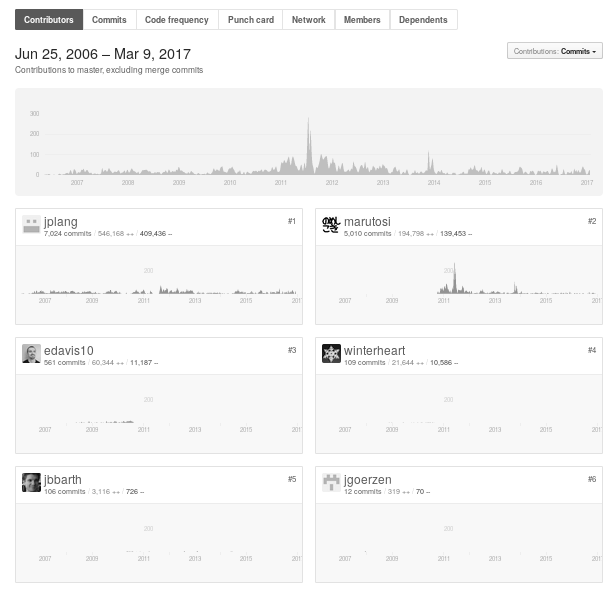
\includegraphics[width=0.8\linewidth]{./chapter-sugestoes-melhorias-fgrm/img/redmine_contribuidores.png}
	\caption{Lista de contribuidores do projeto Redmine}
\label{fig:redmine_contribuidores}
\end{figure}

\subsection{Desenho do Questionário}
\label{ssub:sug_melhoria_desenho_questionario}

A fim de coletar a opinião dos participantes foi utilizado um questionário
eletrônico. O questionário foi desenhado com a premissa de ser respondido em um
prazo curto, de preferência entre 5 e 10 minutos. Neste sentido as perguntas
foram organizadas em dois grupos principais. As questões do primeiro grupo têm
por objetivo coletar a opinião dos profissionais sobre a relevância da
recomendação proposta e o grau de dificuldade de implementá-la. As perguntas
foram estruturadas como uma escala de Likert em que o respondente deveria
fornecer o seu nível de concordância para as declarações que lhe são
apresentadas. No segundo grupo estamos interessados na formação de base
(background) dos profissionais. Optamos por definir algumas das questões como
não obrigatórias por entendermos que a impossibilidade ou falta de interesse em
responder determinada pergunta impeça o participante de enviar os dados de
outras que foram respondidas. O formulário utilizado para coletar os dados dos
participantes pode ser visto no Anexo~\ref{ch:app-form-sug-melhorias}.

\subsection{Processo de Aplicação}
\label{ssub:processo_de_aplicação}

O questionário foi encaminhado à amostra de interesse através de correio
eletrônico. O endereço foi coletado diretamente do projeto hospedado no Github.
Foi desenvolvido um \textit{script} na linguagem Python que permitia coletar o
endereço de e-mail e automatizar o processo de envio. As mensagem foram
personalizadas de modo a identificar o nome do usuário e o projeto do Github com
base no template exibido a seguir. O pedido de participação foi enviado para uma
amostra de 121 contribuidores.

\fbox{\begin{minipage}{\textwidth}
Dear \{\{real\_name \}\}!

I’m conducting a research supervised by Rodolfo Resende \@-\@
homepages.dcc.ufmg.br/~rodolfo and we want to evaluate a collection of
recommendations to new features in Issue Tracking System. As part of them, we
planned and executed a survey aiming at to reach a large-scale population of
practitioners interested in to improve the features of that type of tool. Based
on your area of interest, we kindly invite you to take part in the following
survey:

\{\{url\_formulario\}\}

You were chosen because your contribution in the project \{\{nome\_grupo\}\}
\@-\@ \{\{url\_grupo\}\} hosted on the Github platform. Your opinion is
essential to strength our findings. Please, help us answering this survey until
May 05th. It takes 05 minutes. As soon as we conclude the data analysis, we will
share the results with all participants and the software engineering community.
If you have already fulfilled this questionnaire, please ignore this email.

Thanks in advance,
Vagner Clementino.

\end{minipage}}

O processo de envio consistia ainda de uma segunda mensagem de ``lembrete'' após
dois dias. Esta estratégia foi adotada com base em estudos que discutem
resultados em que o reenvio pode ser um dos fatores que aumentem a taxa de
participação em levantamentos por questionários realizados através da
web~\cite{fan2010factors}.

\section{Resultados da Avaliação das Sugestões de Melhorias}
\label{sec:resultados_avaliacao_sug_de_melhorias}

Após o envio do formulários aos participantes obtivemos um total de 29
respostas. O nível participação foi similar ao observados em outros estudo em
Engenharia de Software que um utilizam o levantamento por questionário (survey)
como método de coleta de dados~\cite{fan2010factors}. Nas próximas seções
apresentamos os resultados obtidos através do perfil dos participantes, a
relevância das sugestões propostas e o grau de facilidade de implementação das
mesmas.

\subsection{Perfil dos Participantes}
\label{sub:sug_melhorias_resultados_perfil_dos_participantes}

\subsection{Relevância das Sugestões}
\label{sub:sug_melhorias_resultados_relevancia}

\subsection{Implementação das Sugestões}
\label{sub:sug_melhorias_resultados_implementacao}

\section{Discussão}
\label{sec:sug_melhoria_discussao}

Acreditávamos que a escolha de N elementos envolveria as principais
características, mas existe possibilidade de ficar alguma característica
relevante fora dos N elementos infelizmente, posteriormente, descobrimos que
ficaram de fora algumas características\dots

\section{Ameaças à Validade}
\label{sec:sug_melhoria_ameacas}

Foco em gente[contribuidores] que trabalha com ferramentas que são
``mainstream'' e portanto têm o viés de visão mais ``tradicional'' (ou outras
caracterizações que podem ser defendidas)

Ao utilizarmos apenas projetos públicos hospedados no Github pode ter causado
algum tipo de direcionamento, como por exemplo foco em projetos de código
aberto. Além disso, não há garantidas que os critérios utilizados para seleção,
como por exemplo seis meses de desenvolvimento ou ter no mínimo 200 revisões
(commits), não nos permite afirmar que escolher os projetos mais
representativos para o nosso público-alvo.

Se (i) escrevermos de maneira extensa a explicação corremos o risco do sujeito
não ler e não responder. Se (ii) escrevermos de maneira ``concisa'' corremos o
risco de ficar vago e não sei se por causa disso ele deixaria de responder.

\section{Resumo do Capítulo}
\label{sec:sug_melhoria_resumo}
